
%TODO refer to the error analysis instead to show that these types of errors are reduced by BSC-Seq.
% \begin{figure*}[t]
% \centering
% \subfloat[Annotator accuracy bias]{
%   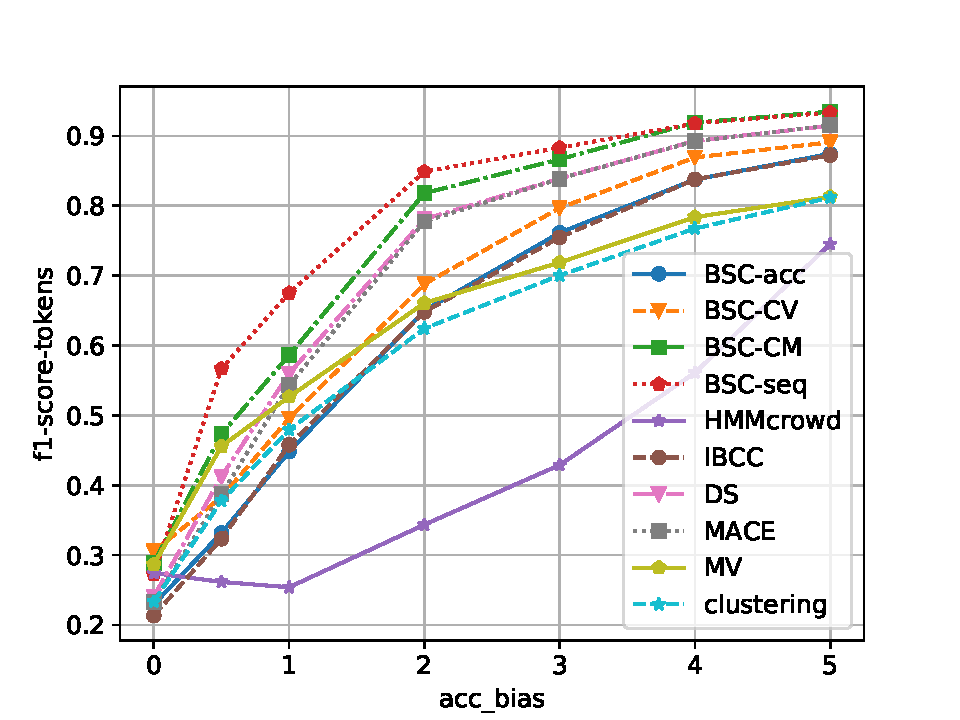
\includegraphics[width=0.505\columnwidth, clip=True, trim=0 20 45 40]{figures/synthetic/acc_bias_exp/plot_f1-score-tokens}
% }
% \subfloat[Short span bias]{
%   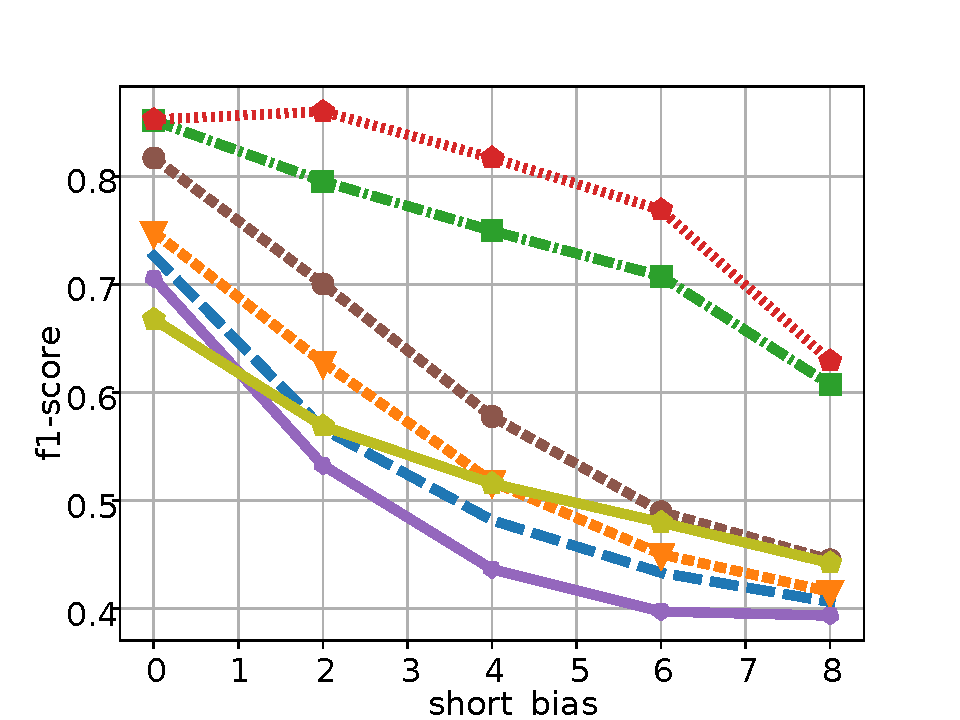
\includegraphics[width=0.485\columnwidth, clip=True, trim=24 18 40 40]{figures/synthetic/short_bias_exp/plot_f1-score-tokens}
% }
% \subfloat[Missed span bias]{
%   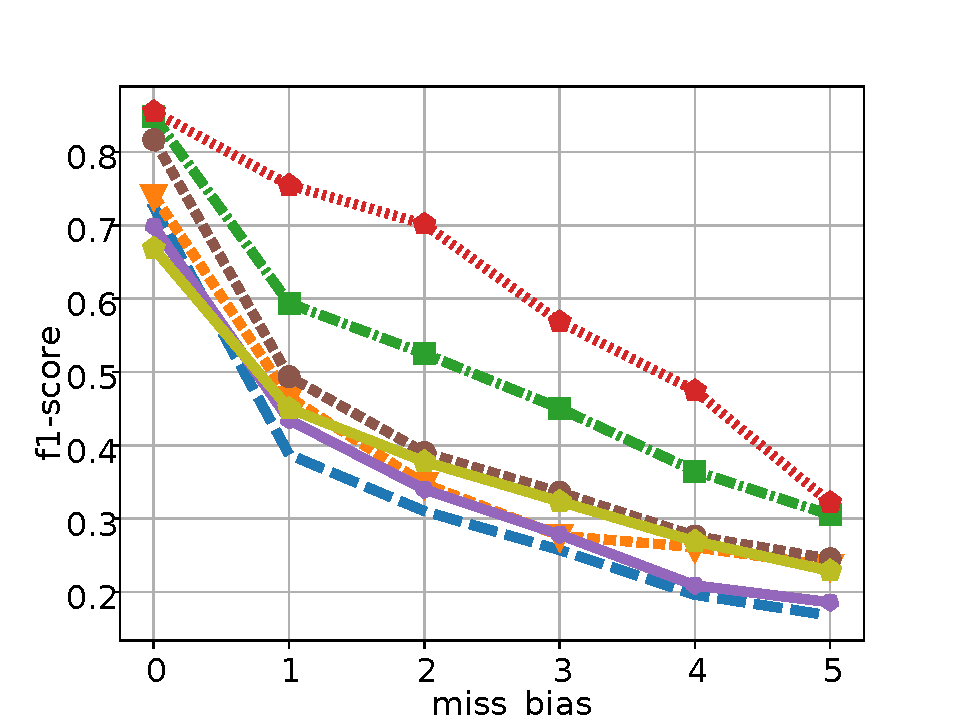
\includegraphics[width=0.485\columnwidth, clip=True, trim=24 18 45 40]{figures/synthetic/class_bias_exp/plot_f1-score-tokens}
% }
% % \subfloat[Crowd size]{
% %   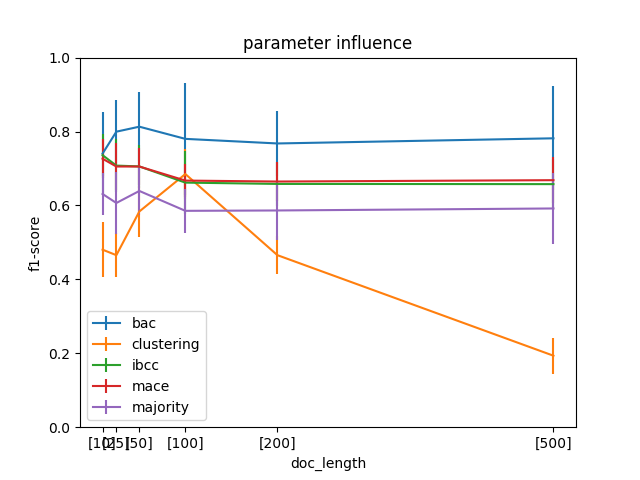
\includegraphics[width=0.2\textwidth, clip=True, trim=0 10 0 27]{figures/synthetic/acc_bias_exp/plot_f1-score.png}
% % }
% \subfloat[
% Good workers out of 10 %a crowd of , where the rest are random.
% ]{
%   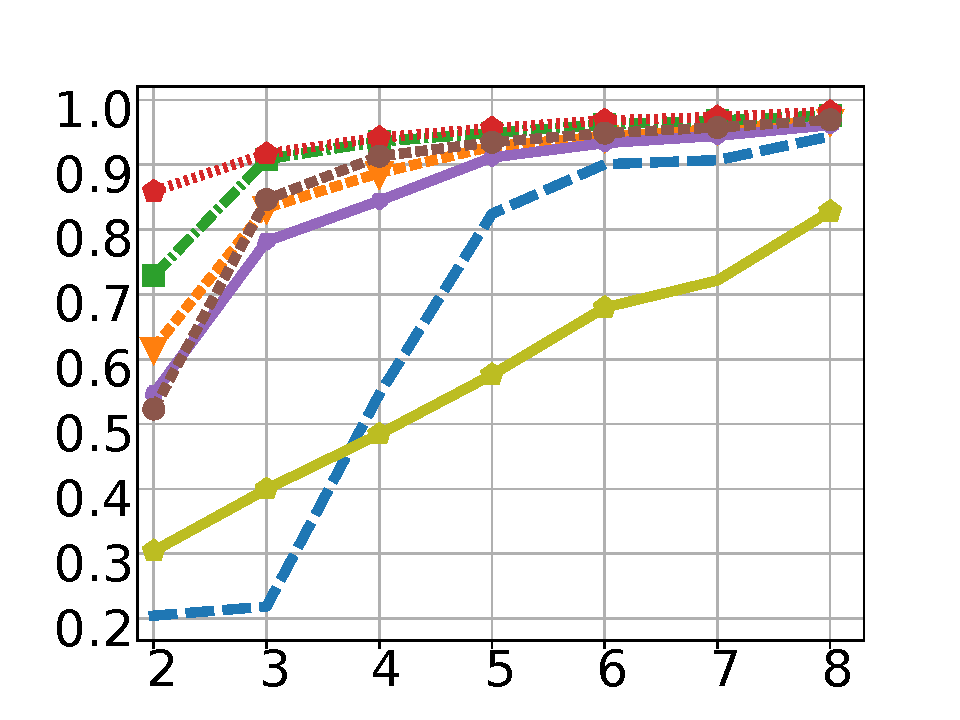
\includegraphics[width=0.485\columnwidth, clip=True, trim=24 18 40 40]{figures/synthetic/group_ratio_exp/plot_f1-score-tokens}
% }
% \caption{F1 scores with simulated annotators. Each plot shows the effect of varying one characteristic.}
% \label{fig:simulated}
% \end{figure*}

\section{Experiments}\label{sec:expts_all}

\begin{table*}[t]
\small
% \begin{tabularx}{\textwidth}{ X X X X X X l l l X X X X} \toprule
% Data & \multicolumn{3}{c}{Sentences with crowd} & \multicolumn{2}{c}{without crowd} & Tokens & \multicolumn{2}{c}{Annotators} & Span & Gold & \multicolumn{2}{c}{Span length}  \\
% -set & total & dev & test & dev & test %crowd & 
% & /sent. & total & /doc & type & spans & mean & std.  \\
% \toprule
% NER & 6056 & 2800 & 3256 & 216 & 231 & 13 & 47 & 4.9 & PER & 6282 & 1.19 & 0.49 \\
% &       & & & & & & &  & LOC  & 6482 & 1.73 & 0.57\\
% &       & & & & & & & & ORG  & 5789 & 1.55 & 0.92\\
% &       & & & & & & & & MISC & 3059 & 1.44 & 0.80\\ \midrule
% PICO & 9480 & 191 & 191 & 191 & 191 & 150 & 312 & 6.0 & pop. & 700 & 7.74 & 7.38  \\ \bottomrule
% \end{tabularx}
\begin{tabularx}{\textwidth}{ X X X X X X l l l X X X X} \toprule
Data & \multicolumn{3}{c}{Sentences with crowd} & \multicolumn{2}{c}{without crowd} & Tokens & \multicolumn{2}{c}{Annotators} & Gold & \multicolumn{2}{c}{Span length}  \\
-set & total & dev & test & dev & test %crowd & 
& /sent. & total & /doc & spans & mean & std.  \\
\toprule
NER & 6056 & 2800 & 3256 & 216 & 231 & 13 & 47 & 4.9 & 21612 % mean per type (std) 5403 (1376) 
& 1.51 & 0.75 \\
PICO & 9480 & 191 & 191 & 191 & 191 & 150 & 312 & 6.0 & 700 & 7.74 & 7.38  \\ \bottomrule
\end{tabularx}
\label{tab:datasets}
\caption{Numbers of sentences, annotators, and spans for datasets used in our experiments. Sentences with crowd all have crowdsourced labels. Only dev and test sentences have gold sequence labels.}
\end{table*}
We evaluate Bayesian sequence combination (BSC) with each of the 
annotator models described in Section \ref{sec:model}
to assess whether the sequential annotator model, \emph{seq},
improves the quality of the inferred sequence tags. 
% (b) the performance of BSC on unreliable or small training sets,
The first experiment uses simulated annotators to investigate the effects of different 
types of error on aggregation methods.
We then introduce two NLP datasets to 
test performance in passive and active learning scenarios, 
analyze errors, and
visualize the learned annotator models.
The experiments also assess whether including including sequence taggers into the probabilistic model
improves the aggregated sequence tags 
as well as the sequence taggers' predictions on test data.
% , and whether 
%models 
%and test LSTM 
%sequence taggers~\cite{lample2016neural}
%trained using our proposed method.

% We further test whether Bayesian approach facilitates more efficient active learning of sequential annotations from crowds and whether integrating the LSTM into the ensemble of annotators improves performance further.
% Our experiments consist of three tasks: (1) aggregating crowdsourced labels, (2) training the LSTM sequence tagger of Lample et al. ~\shortcite{lample2016neural} using aggregated labels, and (3) actively selecting batches of documents for crowdsourced annotation.

\subsection{Evaluated Methods}
As well-established non-sequential baselines, we include token-level majority voting (\emph{MV}), \emph{MACE}~\cite{hovy2013learning}, Dawid-Skene (\emph{DS})~\cite{dawid_maximum_1979} and independent Bayesian classifier combination (\emph{IBCC})~\cite{kim2012bayesian}, a Bayesian treatment of Dawid-Skene. 
We also test the sequential \emph{HMM-crowd} method \cite{nguyen2017aggregating}, which uses a combination of 
maximum \emph{a posteriori} (or smoothed maximum likelihood) estimates for the confusion vector (CV) annotator model 
and variational inference for an integrated hidden Markov model (HMM). 
%  HMM-crowd is the current state-of-the-art and allows us to compare our approach against 
%  a model without a fully Bayesian treatment. 
%We also introduce a \emph{clustering} baseline,
%that aggregates spans from multiple annotators by grouping them together
%using kernel density estimation~\cite{rosenblatt1956remarks}.
MACE and IBCC are variants of BSC-MACE and BSC-CM, respectively, with non-sequential true label models.
%and serve to show the benefits of the sequential BSC model.
HMM-Crowd and DS use non-Bayesian inference steps and can be compared with
their Bayesian variants, BSC-CV and IBCC, respectively. 

BSC is tested with each of the different annotator models described in Section \ref{sec:annomodels}.
%  and two black-box sequence taggers. 
% As the default for all annotator models, 
% we integrate a simple black-box classifier
% that treats all text features as conditionally independent of each other and of the sequence of labels. 
To determine the effect of each component of the model we also test BSC-CM 
and BSC-seq without a text model (\emph{notext}), 
and with the transition matrix, $\bs T$, replaced by simple independent class probabilities (labeled $\backslash \bs T$).
We also test the the BiLSTM-LSTM-CRF of Lample et al.~\shortcite{lample2016neural} 
% as a black-box sequence tagger, labeled \emph{BSC-seq+LSTM}.
% This ensemble is compared against the same LSTM-based method 
trained on the output predictions of HMM-crowd and BSC-seq (labeled $\Arrow{0.2cm}$LSTM).
We use the implementation of Lample et al.~\shortcite{lample2016neural}, which
must be trained on discrete labels and outputs discrete predictions rather than probabilities.
We follow the authors' recommendations for hyperparameters except for the optimizer, 
for which we use Adam to improve the convergence rate as recommended by Reimers and Gurevych~\shortcite{reimers2017optimal}.

% TODO: consider removing prec and rec to make space for the argumentation results.
% Alternatively, the hyper-parameters can be moved elsewhere, but possibly need a simpler setting used for all variants of each model + explanation of why only weak priors were used.
% \subsection{Simulated Annotators}\label{sec:synexpts}
\begin{table*}
\small
\nprounddigits{1}
\npdecimalsign{.}
\begin{tabularx}{\textwidth}{p{3.05cm} X X X X P{0.27cm} P{0.27cm} P{0.27cm} X X X X P{0.27cm}  P{0.27cm}  P{0.27cm} }

%n{2}{1} | n{2}{1} | n{2}{1} | n{2}{1} h Y | Y  | Y  ?  n{2}{1} | n{2}{1} | n{2}{1} | n{2}{1} h Y  | Y  | Y ?}
\toprule
%NER & \multicolumn{3}{|l|}{Span-level metrics}                     & \multicolumn{2}{|l|}{Token-level metrics} & Hyper.\\ \hline 
& \multicolumn{4}{l}{NER} & \multicolumn{3}{l}{Hyperparams.} & \multicolumn{4}{l}{PICO} & \multicolumn{3}{l}{Hyperparams.} \\
& \text{Prec.} &  \text{Rec.} & \text{F1} & \text{CEE} & $\gamma_0$ & $\epsilon_0$ & $\alpha_0$ & \text{Prec.} & \text{Rec.} & \text{F1} & \text{CEE} & $\gamma_0$ & $\epsilon_0$ & $\alpha_0$ \\ \toprule

Best worker & 76.4 & 60.1 & 67.3 & %69.1 & .8521 & 
17.1  & & & &
64.8 & 53.2 & 58.5 & 17.0 & & & \\
Worst worker & 55.7 & 26.5 & 35.9 & %43.5 & .6924 & 
31.9  & & & & 
50.7 & 52.9 & 51.7 & 41.0 & & &\\ \midrule

MV & 79.9 & 55.3 & 65.4 & %69.2 & .9422 & 
6.24  & & & & 82.5 & 52.8 & 64.3 & %76.4 & .923 &
 2.55  & & & \\ 
%MV$\Arrow{0.2cm}$LSTM & 81.2 & 58.7 & 68.1 & %71.0 & .8447 & 
%16.30 & 2 & \\ 
MACE & 74.4 & 66.0 & 70.0 & 1.01 &  .1 & .1 & 0  & 25.4 & 84.1 & 39.0 &% 44.3 & .840 &
 58.2 & .1 & .1 & 0 %72.5 & .8300 & 
\\ 
DS & 79.0 & 70.4 & 74.4 & %76.9 & .9516 & 
2.80 & & & & 71.3 & 66.3 & 68.7 &% \textbf{79.3} & .934 &
 0.44 & & & \\ 
IBCC & 79.0 & 70.4 & 74.4 & %77.1 & .9550 & 
\textbf{0.49} & .1 & 1 & .1 & 72.1 & 66.0 & 68.9 & %\textbf{79.3} & .935 & 
\textbf{0.27} & .1 & 10 & 10\\ 
%IBCC$\Arrow{0.2cm}$LSTM & 79.8 & 67.6 & 73.2 & %74.2 & .9040 & 
%14.01 & 86 & .1, 1, .1 \\ 
\midrule

HMM-crowd & 80.5 & 69.4 & 74.6 & %77.0 & .9762 & 
1.04 & 0 & .1 & 0 & 76.5 & 66.2 & 71.0 & %77.9 & \textbf{.944} & 
0.79 & .1 & 0 & .001 \\ 
% TODO: make it clear that proposing HMMCrowd->LSTM for the aggregation step is novel
HMM-crowd$\Arrow{0.2cm}$LSTM & 81.8 & 69.5 & 75.2 & %77.3 & .8972 & 
12.2 & 0 & .1 & 0 & 76.5 & 66.5 & 71.2 & %78.2 & .868 & 
13.0 & .1 & 0 & .001 \\ 
\midrule
BSC-acc & \textbf{83.4} & 54.3 & 65.7 & %68.2 & .9610 & 
0.96 & 10 & .1 & 10 & \textbf{89.4} & 45.2 & 60.0 & %74.5 & .9069 & 
1.59 & .1 & .1 & 10 \\ 
BSC-MACE & 67.9 & 74.1 & 70.9 & %71.6 & .9658 & 
0.89 & 10 & 10 & 1 & 46.7 & 84.4 & 60.1 & %68.5 & \textbf{.944} &
 1.98 & .1 & 100 & .1\\ 
 %TODO check whether HMMCrowd used any stopwords etc. 
 %TODO possibly rerun with log probabilities produced by the independent features model instead of using the confusion matrix.
BSC-CV & 81.4 & 64.7 & 72.1 & %75.3 & .9715 & 
0.89 & 10 & 1 & 1 & 74.9 & 67.2 & 71.1 & %77.2 & .936 &
 0.84 & .1 & 1 & .1\\ 
BSC-CM & 79.9 & 72.2 & 75.8 & %77.8 & .9635 & 
1.46 & .1 & 100 & .1 & 60.1 & 78.8 & 68.2 & %74.5 & .9434 & 
1.49 & .1 & 100 & 1 \\ 
BSC-seq & 80.3 & 74.8 & 77.4 & %78.9 & .9598 & 
0.65 & .1 & 1 & 1 & 
72.9 & 77.6 & 75.1 & %57.9 & .9250 & 
1.10 & 100 & 1 & 1\\ \midrule
%TODO: separate this into an ablation study?
%TODO: can we hack together a non-Bayesian version of BSC-seq to go in here too?
%BSC-MACE-notext & 78.9 & 66.2 & 72.0 & 0.71 & 10 & .1 & .1 \\ % seems to imply that the HMM over the sequence labels helps MACE. 
%BSC-CM-notext & 75.0 & 68.8 & 71.8 & 0.75 & .1 & 10 & 1\\ % does it imply that the HMM over the sequence labels is detrimental to IBCC?
BSC-CM-notext & 74.7 & 69.7 & 72.1 & 1.48 & .1 & 1 & .1 & 62.7 & 74.8 & 68.2 & 1.32 & 100 & 100 & .1 \\
BSC-CM$\backslash\bs T$ & 80.0 & 73.0 & 76.3 & 0.99 & .1 & 100 & .1 & 65.8 & 66.7 & 66.2 & 0.28 & .1 & 100 & .1  \\
BSC-seq-notext & 81.3 & 71.9 & 76.3 & 0.52 & .1 & 1 & 1 & *81.2 & *59.2 & *68.5 & *0.73 & .1 & .1 & .1\\ 
BSC-seq$\backslash\bs T$ & 64.2 & 44.4 & 52.5 & 0.77 & .1 & 1 & 1 & *51.2 & *70.4 & *59.8 & *1.04 & .1 & .1 & 1\\\midrule
% TODO: put the -> LSTM bits into their own section?
BSC-seq$\Arrow{0.2cm}$LSTM & %82.5 & 76.0 & 79.1 & 10.4 % scores if testing on dev set at every iteration
80.2 & 75.3 & 77.7 & 11.0 
& .1 & 1 & 1 & 
75.7 & 75.4 & 75.5 & %51.6 & .821 & 
25.5 & 100 & 1 & 1\\ 
\bottomrule
\end{tabularx}
\caption{Aggregating crowdsourced labels: estimating true labels for documents labeled by the crowd.}
\label{tab:aggregation_results}
\npnoround
\end{table*}
% Simulated data allows us to test the effect of one  
% type of error in the crowdsourced data,
% while keeping other characteristics of the data constant.
% This can be seen as a sanity check to ensure that both our model and 
% the proposed inference method can handle certain types of error when we know them
% to be present.
% We generate crowds of 10 annotators for four experiments, which  
% test the effect of varying
% (a) average annotator accuracy,
% (b) short span bias, i.e. the probability of not including the last tokens in a span, 
% (c) missed span bias, i.e. the probability of missing a span entirely,
% and (d) the ratio of good to uninformative annotators in the crowd.
% We simulate annotators using the generative model of BSC-seq, 
% drawing annotator labeling probabilities from Dirichlet distributions. 
% %given the ground truth label and the annotator's previous label.
% By default, Dirichlet parameters corresponding to incorrect answers are 1,
% those for correct answers are 2.5, and disallowed transitions (O$\Arrow{0.2cm}$I) are close to 0. 
% We then change the parameters of these Dirichlet distributions 
% to obtain the variations described above. 
% We repeat each experiment 25 times, in each case generating 25 documents of 100 tokens each. 
%
% Figure \ref{fig:simulated} shows the F1-scores for our tested methods. 
% Where annotator accuracy is high, majority voting is less accurate than  methods that model individual annotator behavior, although the difference decreases as we introduce more errors.
% Among the BSC variants, performance increases with the complexity of the annotator model, from BSC-acc to BSC-seq,
% suggesting that the richer seq model can be successfully learned on a small dataset. 
% There are some benefits for the Bayesian approaches, IBCC and BSC-CV, over the similar  models, DS and HMM-crowd, respectively, in handling all four types of annotator error.
% This experiment on simulated data showed that our inference technique was able to handle certain types of error when generated from a BSC model. The following sections
% describe experiments test whether the benefits apply when BSC is used with real crowdsourced data.
% % low annotator accuracy, crowds with few good workers, short span bias and some degree of missed span bias.
% %MACE mostly performs only slightly better than majority vote.
% %, its spammer model
% %handles short span bias and missed span bias relatively well. 
%
%

\begin{figure*}[h]
% \subfloat[BSCC-acc-IF]{
%   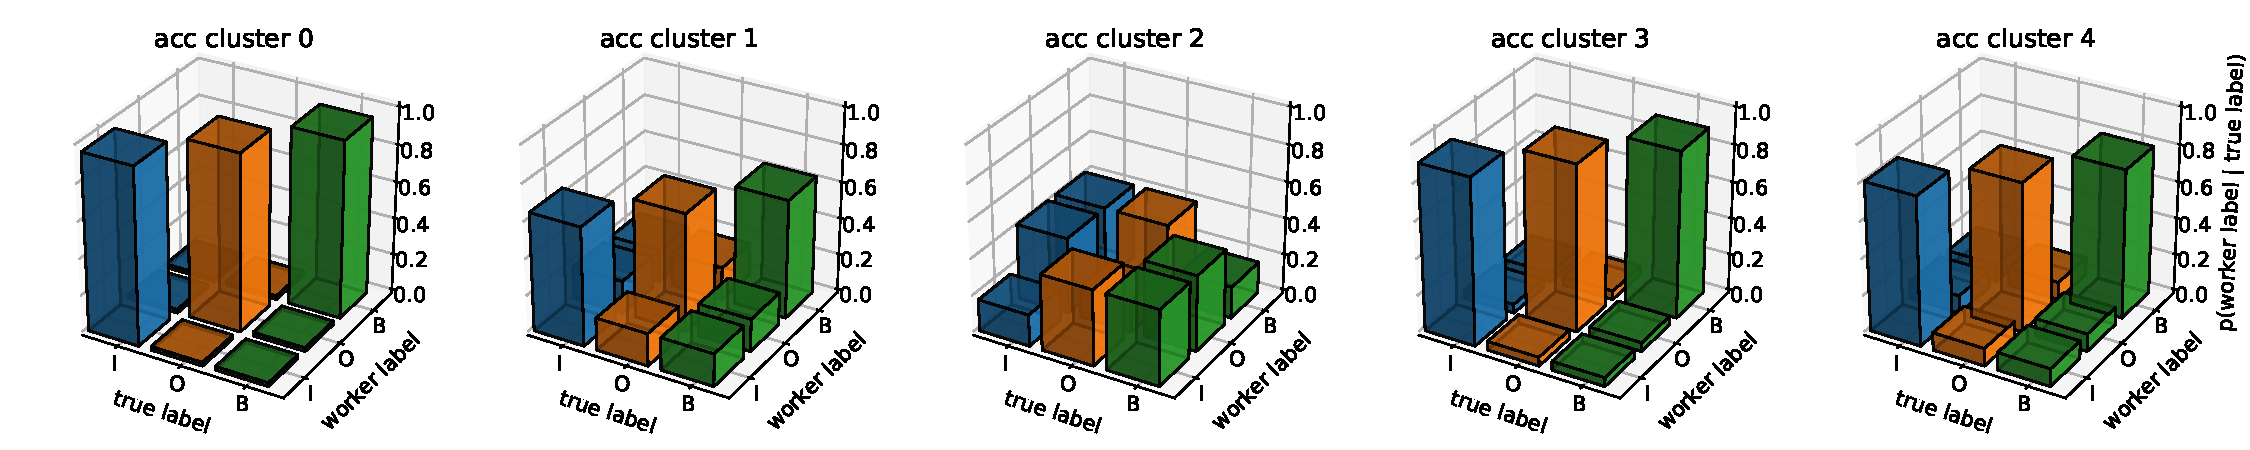
\includegraphics[width=0.9\textwidth, clip=True, trim=0 10 0 28]{figures/worker_models/acc}
% } \\
% \begin{minipage}[b][1cm][l]{0.2\textwidth} 
% BSC-CV:
% \end{minipage}
%   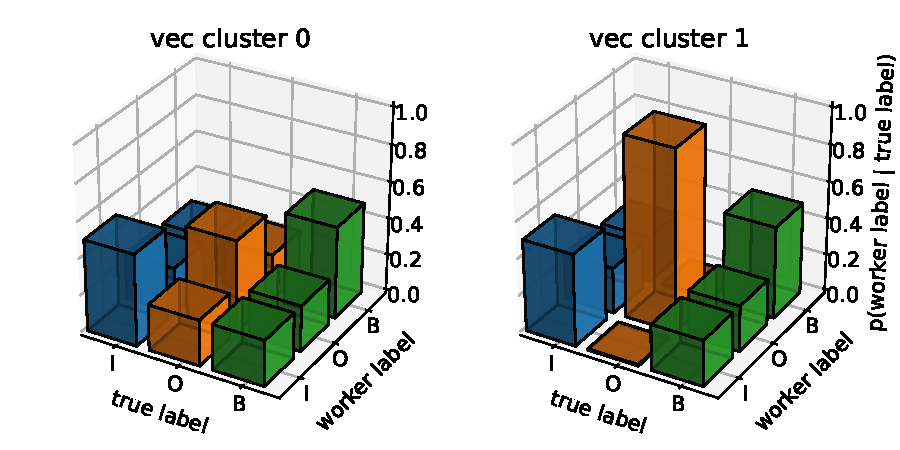
\includegraphics[width=0.72\textwidth, clip=True, trim=0 4 0 3]{figures/worker_models/vec} 
%   \\
% % \subfloat[BSCC-MACE-IF]{
% %   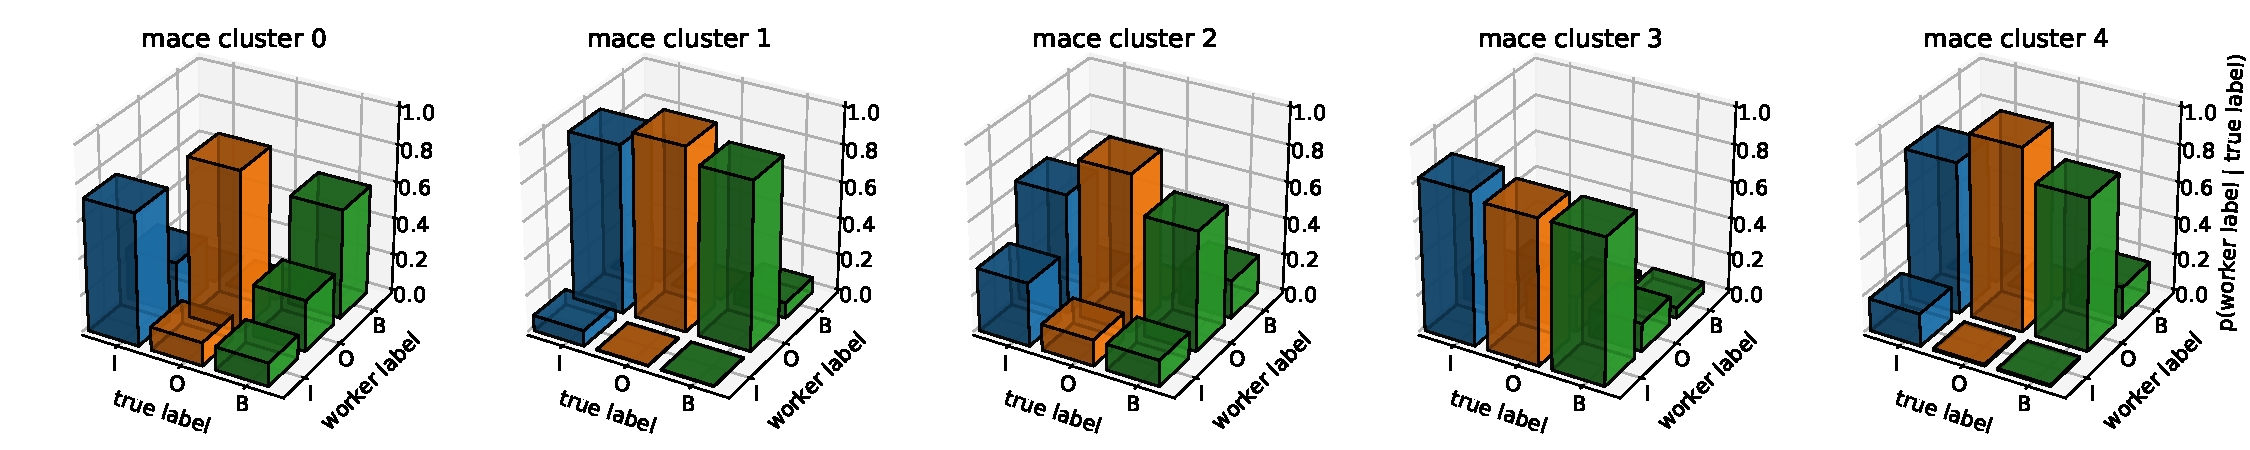
\includegraphics[width=1\textwidth, clip=True, trim=0 10 0 27]{figures/worker_models/mace}
% % } \\
% \begin{minipage}[b][1cm][l]{0.2\textwidth} 
% BSC-CM:
% \end{minipage}
%   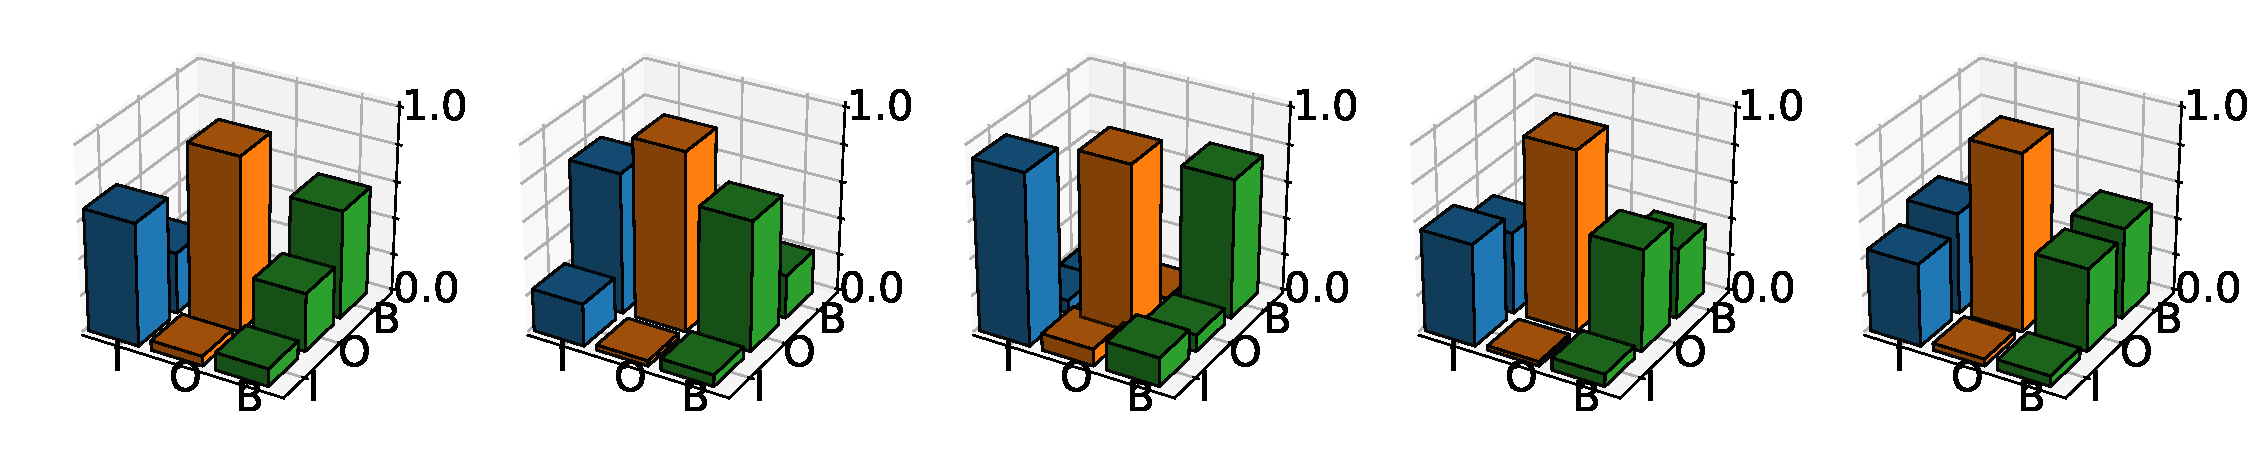
\includegraphics[width=0.7\textwidth, clip=True, trim=20 17 0 28]{figures/worker_models/ibcc}
%  \\
\begin{minipage}[b][1cm][l]{0.2\textwidth} 
BSC-seq, \\
previous label = I:
\end{minipage}
  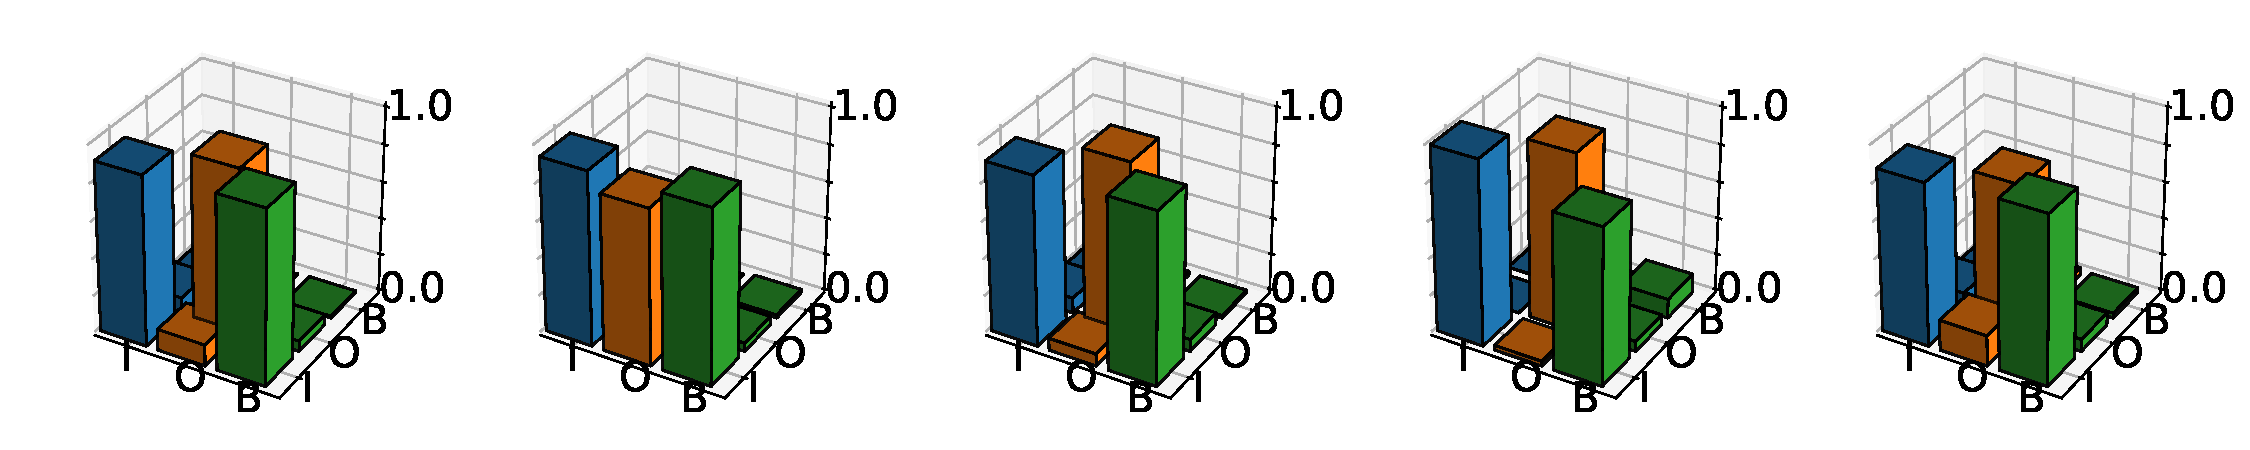
\includegraphics[width=0.7\textwidth, clip=True, trim=20 16 0 28]{figures/worker_models/seq_prev0}
\\
\begin{minipage}[b][1cm][l]{0.2\textwidth} 
BSC-seq, \\
previous label = O:
\end{minipage}
  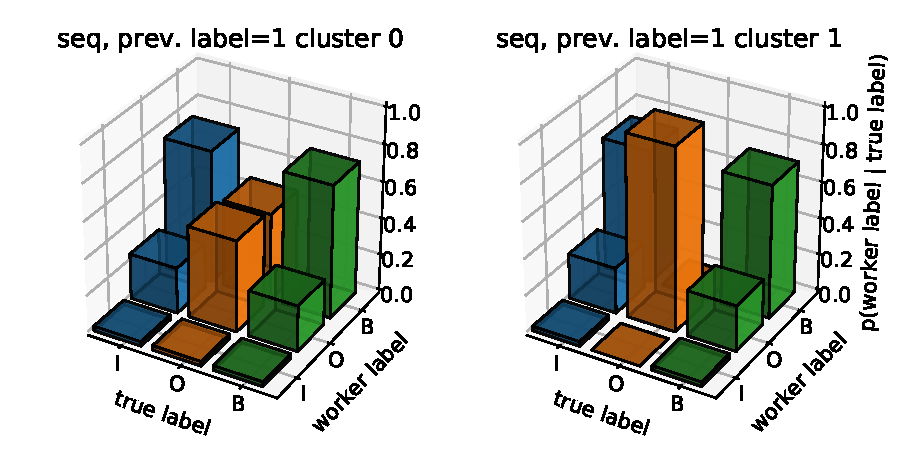
\includegraphics[width=0.7\textwidth, clip=True, trim=20 16 0 28]{figures/worker_models/seq_prev1}
\\
\begin{minipage}[b][1cm][l]{0.2\textwidth} 
BSC-seq,\\
 previous label = B:
\end{minipage}
  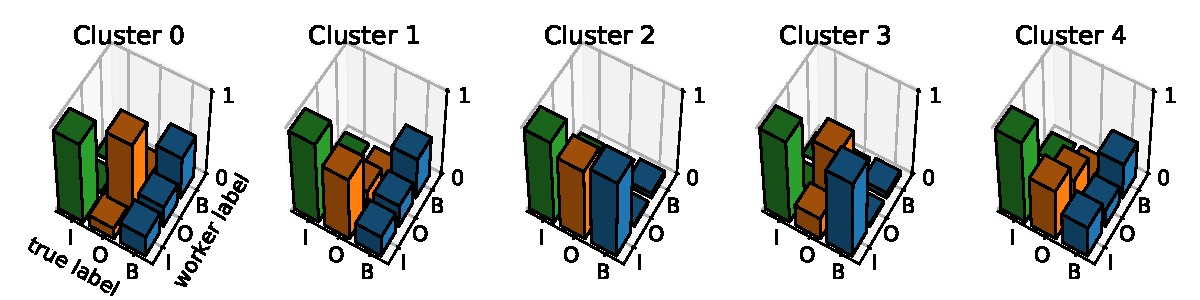
\includegraphics[width=0.7\textwidth, clip=True, trim=20 17 0 28]{figures/worker_models/seq_prev2}
\\
\caption{Clusters of confusion matrix representations from each BSC-*** annotator model trained on PICO. 
}
\label{fig:conf_mat_clusters}
\end{figure*}
%TODO does this need cutting to save space, or moving to the appendix? Possibly the argumentation example would be better. 

\subsection{Crowdsourced Datasets}\label{sec:expts}

We use two datasets containing both crowdsourced and gold sequential annotations. 
The CoNLL 2003 named-entity recognition dataset~\cite{tjong2003introduction},
\emph{NER}, contains gold labels for four named entity categories (PER, LOC, ORG, MISC),
with crowdsourced labels provided by \cite{rodrigues2014sequence}.
\emph{PICO}~\cite{nguyen2017aggregating}, 
consists of medical paper abstracts that have been annotated by a crowd to indicate text spans that identify the population enrolled in a clinical trial. 
Further information about the datasets is shown in Table \ref{tab:datasets}. Note that NER spans are typically much shorter than those in PICO.

\textbf{Evaluation metrics:}
For NER we use the CoNLL 2003 F1-score, which considers only exact span matches %(type, start and end) 
to be correct. 
%This measure is intuitive because complete named entities must be marked to be of value. 
For PICO, we use the relaxed F1-measure~\cite{nguyen2017aggregating}, which counts the matching fractions of spans when computing precision and recall.
Since the spans in PICO are longer than those of NER, partial matches may still contain much of the required information. 
%We additionally compute the root mean squared error in the span lengths, i.e. the difference between the  % actually it's not quite that. We computed the difference in mean span lengths. This is already captured by F1 score for pico and better described by the span-level-precision and recall. Our metric might be more if we didn't take the absolute so we could see if spans were often too long or too short.
We also compute the cross entropy error (\emph{CEE}) at the level of tokens
to compare the probability estimates produced by aggregation methods, which are useful for decision-making tasks such as active learning.


\subsection{Aggregating Crowdsourced Labels}\label{sec:task1}

In this task, we use the aggregation methods to combine multiple crowdsourced labels and predict the true labels for the same documents. 
For both datasets, we provide all the crowdsourced labels as input to the aggregation method. 
In both cases, we split the gold-labeled documents into 50\% validation and test sets. 
For NER, we use the split given by Nguyen et al. ~\shortcite{nguyen2017aggregating},
while for PICO, the split was not available so our results are not directly comparable to theirs.

We tune the hyperparameters using a validation set. To limit the number of hyperparameters to tune, we optimize only three values for BSC.
Hyperparameters of the transition matrix, $\bs\gamma_j$, are set to the same value, 
$\gamma_0$, except for disallowed transitions, (O$\Arrow{0.2cm}$I, transitions between types, e.g. I-PER$\Arrow{0.2cm}$I-ORG), which are set to 0.1.  
For the annotator models (both $\bs A$ and $\bs B$),
all values are set to $\alpha_0$, except for disallowed transitions, which are set to 0.1, then $\epsilon_0$ is added to hyperparameters 
corresponding to correct annotations (e.g. diagonal entries in a confusion matrix).
We use $\epsilon_0$ to encode the prior assumption that annotators are more likely to have an accuracy greater than random. This avoids the non-identifiability problem, in which the class labels become switched around.
We use validation set F1-scores to choose values from $[0.1, 1, 10, 100]$, 
training on a small subset of 250 documents for NER and 500 documents for PICO. 
% For the integrated BSC-seq+LSTM,  
% we found better validation set performance for both our datasets if the LSTM is first excluded while 
% the other parameters converge before training the LSTM. 
% This simply means that we follow Algorithm \ref{al:vb_bac}, but omit steps 3, 
% 4 and 6 in the first few iterations.
Note that we use the dev set at each VB iteration to select the best
LSTM model after each epoch. 
%this means that in some iterations, we might reject all the latest epochs so a model would get stuck, potentially in a local maximum. But if we don't do it, we would overshoot the optimum.
% the resolution would be to have multiple epochs per VB iteration, or to keep each LSTM update and
% use the dev set to choose the best VB iteration to stop at.
% These steps reduce over-fitting resulting from the maximum likelihood step used to integrate the LSTM as a black-box sequence tagger.

The results of the aggregation task are shown in Table \ref{tab:aggregation_results}.
Although DS and IBCC do not consider sequence information nor the text itself, 
they both perform well on both datasets,
with IBCC reaching better cross entropy error than DS due to its Bayesian treatment.
%against HMM-crowd on NER,
%and BSC-CM variants on PICO. 
The improvement of DS over the results given 
by Nguyen et al. ~\shortcite{nguyen2017aggregating} may be due to implementation differences. 
Neither MACE, BSC-acc nor BSC-MACE perform strongly, with F1-scores sometimes falling below MV. 
The acc and MACE annotator models may be a poor match for the sequence labeling task if annotator
competence varies greatly depending on the true class label.

%The annotator models of BSC-CV and BSC-CM are better, although BSC-CM performs worse on PICO.
BSC-seq outperforms the other approaches, although 
%despite
%having a larger number of parameters to learn.
without the text model (BSC-seq-notext) or the transition matrix (BSC-seq$\backslash\bs T$),
its performance decreases.
However, for BSC-CM, the results are less clear: BSC-CM-notext differs from IBCC only in the 
inclusion of the transition matrix, $\bs T$, yet IBCC outperforms BSC-CM-notext.
This suggests that the combination of these elements is important: the seq annotator model is effective 
in combination with the transition matrix and simple text model.
Integrating an LSTM improves performance further in both datasets, and outperforms an LSTM trained on the output of HMM-crowd or BSC-seq.

\begin{table*}[h]
\small
\begin{tabularx}{\textwidth}{l X X X X X X X X X X X X}
\toprule
Method & Data-set & exact match & type wrong only & partial match & mis-sing span & false +ve & late start & early start & late finish & early finish & fused spans & split span \\ \midrule
MV & NER & 4307 & 304 & 228 & 1773 & 100 & 96 & 10 & 15 & 85 & 17 & 26 \\
HMM-crowd & NER & 4519 & 361 & 256 & 924 & 182 & 101 & 15 & 26 & 97 & 28 & 22 \\
BSC-CV & NER & 4431 & 275 & 243 & 1245 & 177 & 100 & 17 & 23 & 89 & 29 & 16 \\
BSC-CM & NER & 4534 & 387 & 258 & 734 & 269 & 111 & 23 & 37 & 86 & 39 & 12 \\
BSC-seq & NER & 4581 & 351 & 261 & 564 & 195 & 93 & 42 & 33 & 85 & 39 & 17 
% note this is actually from +LSTM and needs regenerating.
\\
\midrule 
MV & PICO    & 168 & 0 & 32 & 185 & 48 & 9 & 11 & 1 & 0 & 3 & 9 \\
HMM-crowd    & PICO & 190 & 0 & 47 & 124 & 81 & 13 & 21 & 0 & 0 & 5 & 8 \\
BSC-CV       & PICO & 156 & 0 & 76 & 117 & 81 & 10 & 25 & 0 & 0 & 11 & 0 \\
BSC-CM       & PICO & 174 & 0 & 98 & 192 & 18 & 15 & 8  & 0 & 4 & 18 \\
BSC-seq      & PICO & 173 & 0 & 40 & 136 & 56 & 32 & 26 & 23 & 2 & 4 & 10
% BSC-seq+LSTM & PICO & 81 & 0 & 421 & 75 & 216 & 20 & 6 & 232 & 3 & 24 & 393 \\
\bottomrule
\end{tabularx}
\caption{Counts of different types of span errors.}
\label{tab:error_analysis}
\end{table*}
We categorize the errors made by key methods and list the
counts for each category in Table \ref{tab:error_analysis}.
All machine learning methods shown reduce the number of spans that were completely missed by majority
voting. 
% BSC-seq+LSTM increases the number of exact span matches on NER, but reduces this number substantially on PICO
% while increasing the number of partial matches and false positives (where no true span was present). 
% This is due to a larger number of split spans, where a 'B' token is inserted incorrectly inside
% a span. 
% Therefore, while BSC-seq outperforms the alternatives in terms of F1-score and missing spans, 
% further work may be required to improve the distinction between 'B' and 'I' tokens. 

% TODO: make this plot more compact and relevant by plotting only the means across the whole dataset, 
%and the distribution of hellinger distances between the confusion matrices for each previous label case. Put on a single row.
%Table \ref{tab:aggregation_results} shows a benefit of using the sequential annotator model over CM, CV and acc.
To determine whether BSC-seq learns distinctive confusion matrices depending on the previous labels,
we plot the learned annotator models for
PICO as probabilistic confusion matrices in Figure \ref{fig:conf_mat_clusters}.
As the dataset contains a large number of annotators, we clustered 
the confusion matrices inferred by each model
into five groups by applying K-means to their posterior expected values,
then plotted the means for each cluster.
In all clusters, BSC-CV learns different accuracies for B, I and O (the diagonal entries). 
These differences may explain its
improvement over BSC-acc.
BSC-CM differs from BSC-CV in that %has more distinctive clusters and 
the first, fourth and fifth clusters 
have off-diagonal values with different heights for the same true label value.
 The second 
cluster for BSC-CM encodes likely spammers who usually choose 'O' regardless of the 
ground truth. 
%Unlike BSC-CM, BSC-seq improved performance on PICO over BSC-CV. 
The confusion matrices for BSC-seq are
very different depending on the worker's previous annotation. 
Each column in the figure shows the confusion matrices corresponding to the same cluster of annotators. 
The first column, for example, shows
annotators with a tendency toward I$\Arrow{0.2cm}$I or O$\Arrow{0.2cm}$O transitions, while the following clusters 
indicate very different labeling behavior. The model therefore appears able to learn
distinct confusion matrices for different workers given previous labels, which supports the use of sequential
annotator models.

%TODO decide whether this should be kept in to show the value of the uncertainty estimates? If so, merge back into two plots and
% cut the + LSTM result. The method may need changing or checking that it is a sensible strategy for sequences?
% \subsection{Active Learning}
%
% \begin{figure*}[h]
% \centering
% % \subfloat[NER, random sampling]{
% %   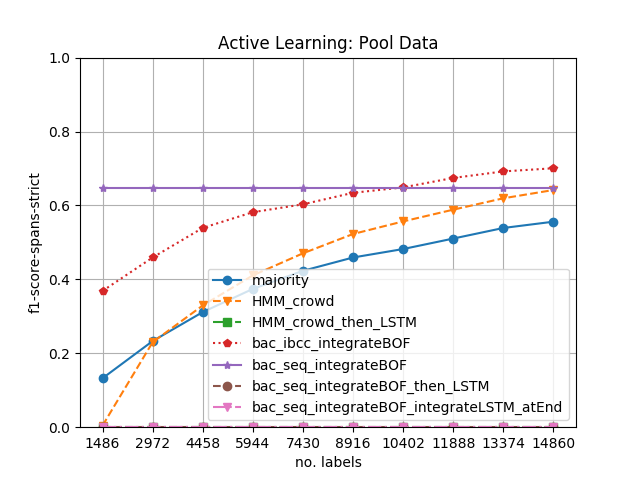
\includegraphics[width=0.9\columnwidth, clip=True, trim=12 0 0 38]{figures/NER_RAND/pool/plot_f1-score-spans-strict}
% % }
% \subfloat[NER]{
%   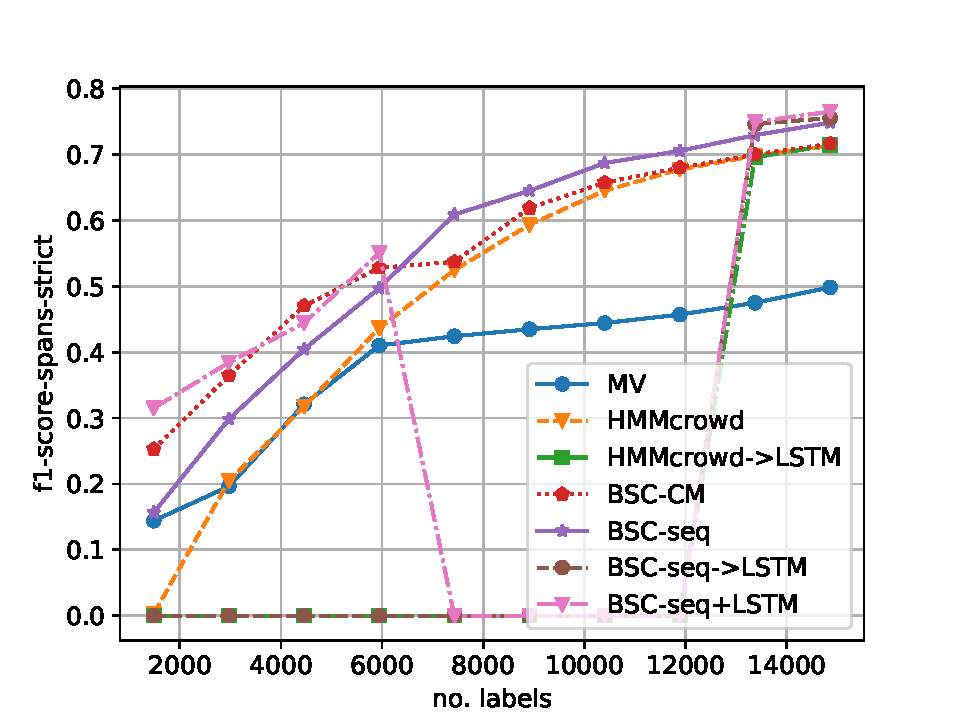
\includegraphics[width=0.518\columnwidth, clip=True, trim=41 22 32 15]{figures/NER_AL/pool/plot_f1-score-spans-strict.pdf}
%   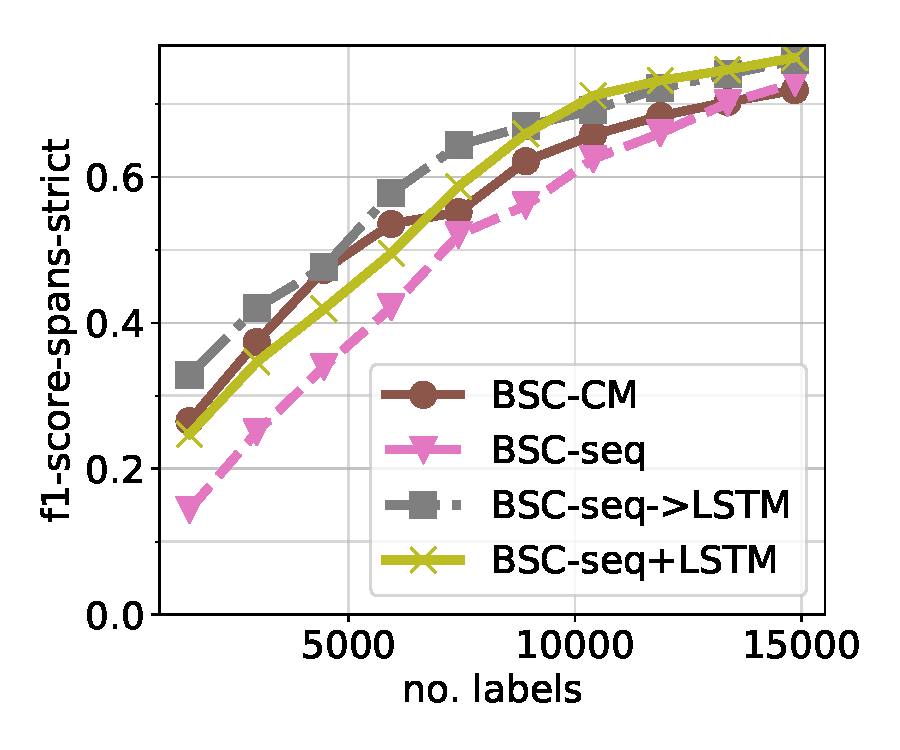
\includegraphics[width=0.469\columnwidth, clip=True, trim=75 22 32 15]{figures/NER_AL/pool2/plot_f1-score-spans-strict.pdf}
% }
% \centering
% % \subfloat[PICO, random sampling]{
% %   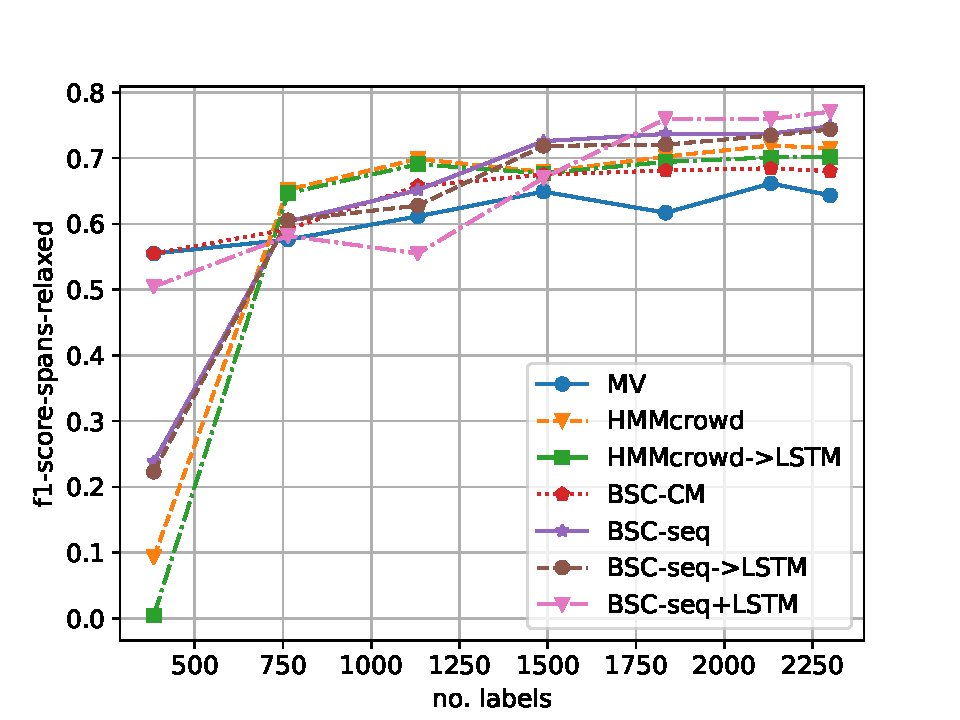
\includegraphics[width=0.9\columnwidth, clip=True, trim=12 0 0 40]{figures/PICO_RAND/pool/plot_f1-score-spans-relaxed}
% % }
% \subfloat[PICO]{
%   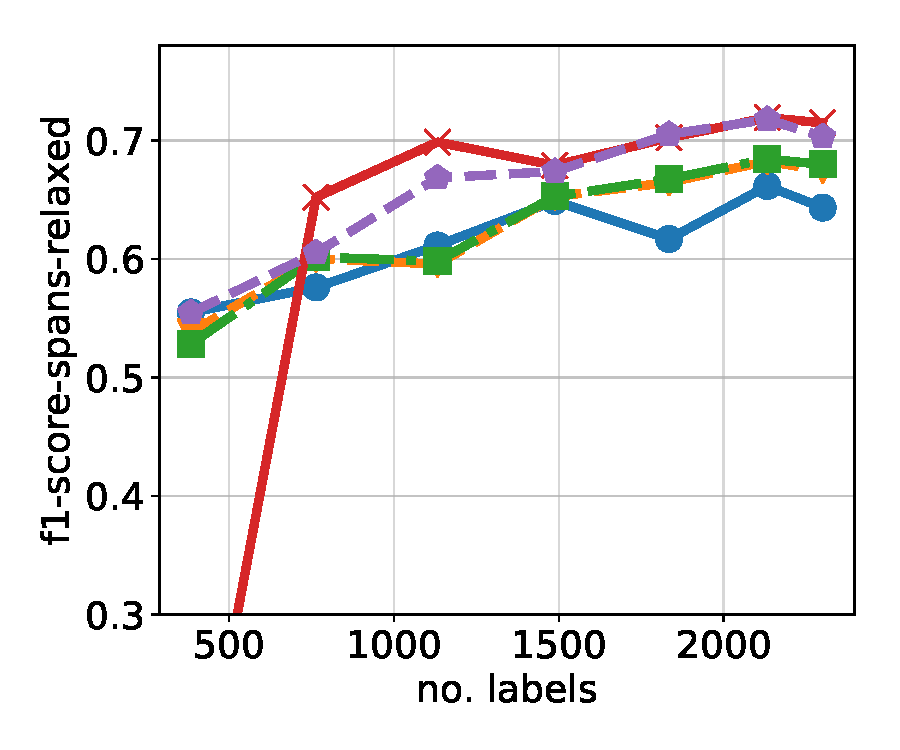
\includegraphics[width=0.53\columnwidth, clip=True, trim=42 22 21 15]{figures/PICO_AL/pool/plot_f1-score-spans-relaxed.pdf}
%   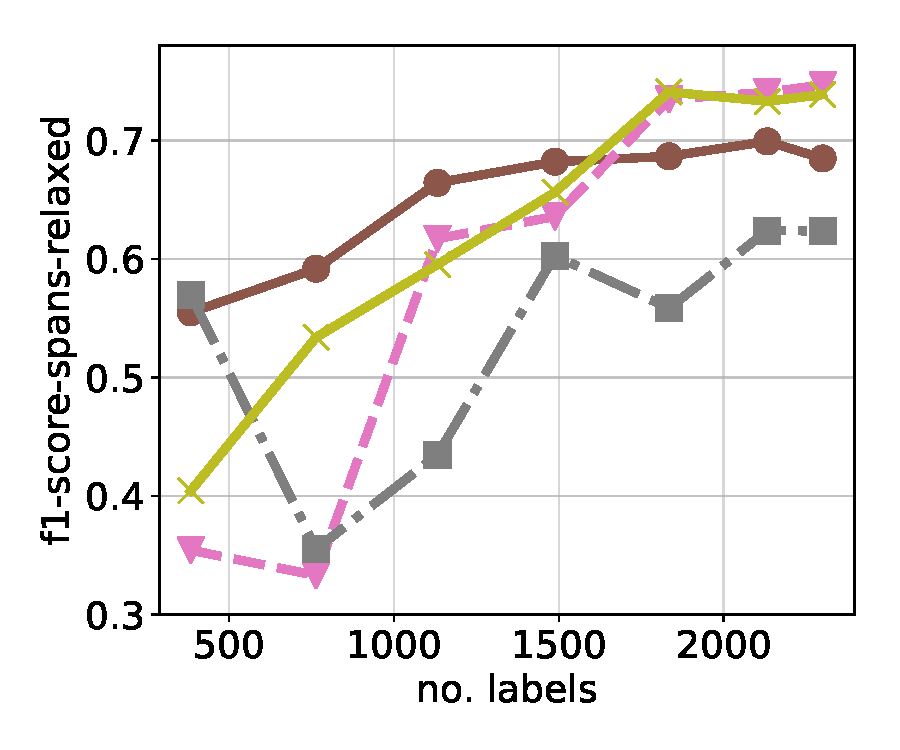
\includegraphics[width=0.483\columnwidth, clip=True, trim=75 22 21 15]{figures/PICO_AL/pool2/plot_f1-score-spans-relaxed.pdf}
% }
% \caption{F1-scores for active learning simulations using uncertainty sampling.
% %: prediction performance after each labelled batch is received. Mean scores over 10 repeats.
% }
% \label{fig:alner}
% \end{figure*}
% Active learning iteratively selects informative data points to be labeled so that a model can be trained
% using less labeled data. Posterior probabilities output by Bayesian methods 
% account for uncertainty in the model parameters, hence can be used to choose data points that rapidly reduce uncertainty. 
% %In contrast, frequentist methods
% %such as maximum likelihood output probabilities that do not account for parameter uncertainty due to 
% %small datasets or noisy labels. 
% We hypothesize that BSC will learn more quickly than non-sequential methods
% in an active learning scenario. 
% %HMMCrowd, which uses only partially-Bayesian
% %inference, and majority voting, which is not probabilistic and also does not benefit from a sequential model.
% %When the labeled dataset is small and many documents have few labels, the integration of an LSTM
% %may improve performance as it acts as an additional annotator.
% %We investigate the performance of the aggregation methods with smaller datasets,
% %and 
% %the effectiveness of active learning at improving performance with fewer annotations.
% %improve the efficiency of the annotation process.
% %Two set-ups were evaluated on NER and PICO: 
% %the first tests our methods on random subsamples of crowdsourced data of increasing size;
% %the second starts with a random initial subsample,
% %To test these hypotheses, we
% While various active learning methods could be applied here, in this paper we wish
% to demonstrate only that BSC may serve as a good foundation for active learning,
% and defer a deeper investigation of active learning techniques to future work.
% We therefore simulate active learning using a well-established technique, \emph{uncertainty sampling}~\cite{settles2008analysis,settles2010active},
% as described in Algorithm \ref{al:uncertainty_sampling}.
% \begin{algorithm}
% \DontPrintSemicolon
%  \KwIn{ A random $initial\_set$ of training labels, the same for all methods. }
%  \nl Set training set $\bs c=initial\_set$ \;
%  \While{training set size < $max\_no\_labels$}
%  {
%  \nl Train model on $\bs c$ \;
%  \nl Predict sequence labels for all documents\;
%  \nl Compute the mean entropy of the sequence labels of each document: 
%  $-\frac{1}{L_n} \sum_{\tau=1}^{L_n}
%  \sum_{j=1}^J
%  p(t_{n,\tau} = j | \bs c) \ln p(t_{n,\tau} = j | \bs c) $
%  \;
%  \nl Select $batch\_size$ documents with highest mean entropy, add their annotations to $\bs c$\;
%  }
% \caption{Active learning simulation for each method using uncertainty sampling.}
% \label{al:uncertainty_sampling}
% \end{algorithm}
% The LSTM implementation provided by Lample et al.~\shortcite{lample2016neural} 
% outputs discrete label predictions, so to allow direct comparison of BSC against a neural sequence tagger,
% we modify the network to output probabilities for the active learning simulation. For MV, probabilities
% are estimated by fractions of votes.
% %Here we compute entropy over token labels independently so that 
% %the method is applicable to non-sequential models such as majority voting. 
% %However, for sequential models such as HMM-crowd and BSC, the entropy 
% %could in future take into account the label dependencies, which may improve performance.
%
% %to iteratively select additional crowd labels given posterior label predictions from a model trained on the previous subset. To compute the uncertainty of each
% %document, we take the mean shannon entropy $H$ of the labels, 
% %
% %We used the same random samples for all methods and repeated 
% %the experiments ten times with different initializations. 
% %\begin{table}
% %\small
% %\begin{tabularx}{\columnwidth}{|l | Y | Y | Y |} \hline
% %No. Tokens & I & O & B \\ \hline
% %1486 & 0.22	& 0.978	& 0.648 \\
% %14860 & 0.502	& 0.819	& 0.612 \\
% %29704 & 0.695	& 0.539	& 0.533 \\ \hline
% %\end{tabularx}
% %\caption{Mean accuracies for the integrated LSTM learned by BSC-seq+LSTM on subsamples of NER. 
% %The accuracy is the probability of correct label given the posterior expectation of the 
% %sequential confusion matrix, averaged over previous label values. 
% %}
% %\label{tab:lstm_accs}
% %\end{table}
% Figure \ref{fig:alner} plots the mean F1 scores over ten repeats of the active learning simulation.
% IBCC learns more rapidly than DS on NER due to its Bayesian approach,
% which may also explain the stronger performance
% of BSC-CV compared to the similar HMM-crowd model, although this does not hold for the PICO dataset.
% BSC variants outperform non-sequential IBCC. BSC-CM and BSC-CV are strongest on PICO with small numbers of labels,
% but are later overtaken by BSC-seq, which may require more data to learn its more complex model.
% On NER, BSC-CM continues to outperform the more complex BSC-seq,
% but the integrated LSTM clearly improves BSC-seq+LSTM.
% %Uncertainty sampling appears to have a greater improvement over random sampling on NER
% %after around $7000$ labels have been obtained, suggesting that a different strategy could be beneficial while
% %the dataset is very small. 
% %On PICO, with its smaller sample sizes, the effect of active learning is only observed
% %with BSC-seq+LSTM.
% BSC-seq$\Arrow{0.2cm}$LSTM performs strongly on NER but poorly on PICO, where fewer labels were provided,
% while BSC-seq+LSTM appears more robust to this problem.  
% %and HMM-crowd$\Arrow{0.2cm}$LSTM are effective on NER with smaller datasets, improving over BSC-seq and HMM-crowd methods that 
% %use only a simple independent text model to make predictions for unlabeled data. 
% %However, on PICO, they underperform BSC-seq and HMM-crowd respectively, possibly because the dataset is too small to train 
% %the LSTM reliably.
% %BSC-seq+LSTM accounts for the unreliability of the predictions of the integrated LSTM, 
% %enabling it to outperform BSC-seq$\Arrow{0.2cm}$LSTM on NER with more than $10000$ labels and on PICO at almost all points.
% %We observe that
% %  BSC-seq$\Arrow{0.2cm}$LSTM learns different values for the accuracy of the integrated LSTM depending on the true class label, even with only 1486 tokens  labeled by the crowd.
%
% %By examining the posterior reliability model for the integrated LSTM learned by 
% %, we observe that 
% %Table \ref{tab:lstm_accs} shows that even for small datasets, BSC-seq+LSTM learns to account for the unreliability
% %of the LSTM itself.
% % The selection method and batch size could be fine-tuned for future applications -- the 
% % goal of our experiment in this paper was to test the benefits of the proposed aggregation methods,
% % rather than to establish a robust active learning approach.
% % BSC-seq+LSTM models the reliability of the integrated LSTM. 
% % Table \ref{tab:lstm_accs} summarises the accuracies learned by the model for each class label
% % on the NER dataset. The differences in the inferred accuracy of the LSTM for each class shows that
% % the model is able to make use
%
\subsection{Prediction with Crowd-Trained LSTMs}\label{sec:task2}

\begin{table*}
%TODO cut out prec and rec to make space for arg? Cut out CEE in this case too, as this is not assessing the Bayesian method.
% Then it can all go in one column and the top line can be cut.
\small
\begin{tabularx}{\textwidth}{ l X X X X X X X X}
\toprule
%PICO & \multicolumn{3}{|l|}{Span-level metrics (std.)}                          & \multicolumn{2}{|l|}{Token-level metrics (std.)} \\ \hline 
 & \multicolumn{4}{l}{NER} & \multicolumn{4}{l}{PICO}\\ 
& Prec. & Recall & F1 & CEE & Prec. & Recall & F1 & CEE  \\ \midrule
HMM-crowd$\Arrow{0.2cm}$LSTM & \textbf{78.7} & 59.0 & 67.5 & 15.9  & \textbf{75.6} & 61.6 & 67.9 & 13.5 \\
BSC-seq$\Arrow{0.2cm}$LSTM & 76.9 & 64.1 & \textbf{69.9} & 14.54 & 82.3 & \textbf{66.4} & \textbf{73.5} & 19.6  \\
LSTM trained on gold & 77.6 & 75.3 & 76.5 & 11.10 & \multicolumn{4}{l}{too few training labels} \\
\bottomrule
\end{tabularx}
\caption{Prediction performance on test datasets with training on crowdsourced labels.}
\label{tab:prediction_results}
\end{table*}
In previous work~\cite{nguyen2017aggregating}, HMM-crowd$\Arrow{.2cm}$LSTM
produced better predictions for documents not labeled by the crowd, compared with 
training an LSTM directly on crowdsourced data, or training
on labels obtained from non-sequential aggregation methods. 
We evaluate whether the performance gains of BSC-seq$\Arrow{.2cm}$LSTM for aggregation also result in better predictions 
on unannotated documents. 
% We also test whether 
% BSC-seq+LSTM can provide meaningful 
% confidence estimates when the sequence tagger it integrates produces only discrete labels.
% we used the dev sets to do early stopping. Should we also say that we tuned hyperparameters on 2002 data?
% ideally we should tune the hyperparameters of each of these instances separately on the dev set OR
% assume there is no dev set in this scenario so we have to either split one off or use settings from another dataset.
% I think this applies equally to the previous scenario. It makes most sense if another dataset is used for dev, and
% no early stopping is applied.
%We compare the Bi-LSTM-LSTM-CRF sequence taggers~\cite{lample2016neural}
%trained by HMM-crowd and BSC-seq on test data from NER and PICO. 
For NER, we evaluate on the CoNLL English test set~\cite{tjong2003introduction}.
%while for PICO, we train the aggregators on the $3,649$ documents without gold labels, 
%then evaluate on the gold-labelled test data split used in Section \ref{sec:task1}.

The results in Table \ref{tab:prediction_results} show that for F1-scores, BSC-seq$\Arrow{.2cm}$LSTM 
outperforms 
the previous state-of-the-art, HMM-crowd$\Arrow{.2cm}$LSTM.
%F1-scores  for BSC-seq+LSTM are lower than those of BSC-seq$\Arrow{0.2cm}$LSTM,
%although it also outperforms
%HMM-crowd$\Arrow{0.2cm}$LSTM.
% BSC-seq+LSTM produces a low cross entropy error, 
% indicating that the probabilities it outputs are a good reflection of confidence and
% are likely to be more suitable to downstream decision-making tasks than the raw outputs
% from the LSTM sequence tagger.  
%The benefits of Bayesian ensemble methods
%such as BSC for decision-making tasks is therefore a promising topic for future work.
%This suggests that the strength of our technique for 
%integrating sequence taggers comes from 
%combining the LSTM with human annotators, as in Section \ref{sec:task1}.
%The same technique can also be used to combine multiple sequence taggers in an ensemble,
%which may be an avenue for future work.
